\باب{مقناطیسی قوتیں، مقناطیسی مادے اور امالہ}
برقی چارج کے گرد برقی میدان پایا جاتا ہے جس میں موجود ساکن یا حرکت کرتے چارج پر قوت دفع یا قوت کشش پایا جاتا ہے۔مقناطیسی میدان برقی رو یعنی حرکت کرتے چارج سے پیدا ہوتا ہے اور اس میدان میں حرکت کرتے چارج پر قوت پائی جاتی ہے۔مقناطیسی میدان ساکن چارج پر قوت پیدا نہیں کرتا۔

اس باب میں برقی رو گزارتی تار پر قوت اور مروڑ  کا جائزہ لیا جائے گا۔ اس کے بعد مقناطیسی اشیاء اور آخر میں امالہ پر غور کیا جائے گا۔

\حصہ{متحرک چارج پر قوت}
تجربے سے  ثابت ہوتا ہے کہ برقی میدان میں چارج بردار ذرے  پر 
\begin{align}\label{مساوات_امالہ_برقی_قوت}
\kvec{F}=Q \kvec{E}
\end{align}
قوت اثر انداز ہوتی ہے۔مثبت چارج کی صورت میں یہ قوت برقی میدان کے شدت \عددیء{\kvec{E}} کی سمت میں ہوتی ہے۔قوت کی قیمت چارج \عددیء{Q} اور برقی میدان کی شدت \عددیء{\kvec{E}} کے حاصل ضرب کے برابر ہوتی ہے۔چارج ساکن ہو یا حرکت کر رہا ہو، اس پر قوت کی مقدار اسی مساوات سے حاصل ہوتی ہے۔

اسی طرح تجربے سے ثابت ہوتا ہے کہ مقناطیسی میدان میں ساکن چارج بردار ذرے  پر مقناطیسی میدان کوئی قوت پیدا نہیں کرتا البتہ متحرک چارج بردار ذرے  پر مقناطیسی میدان
\begin{align}\label{مساوات_امالہ_مقناطیسی_قوت}
\kvec{F}=Q \kvec{v} \times \kvec{B} 
\end{align}
قوت پیدا کرتا ہے۔یہ قوت چارج  کے براہ راست متناسب ہوتی ہے۔اسی طرح قوت چارج کے رفتار \عددیء{\kvec{v}}،  کثافت مقناطیسی میدان \عددیء{\kvec{B}} اور ان دو کے مابین زاویے کے سائن کے بھی براہ راست متناسب ہوتی ہے۔قوت کی سمت \عددیء{\kvec{v}} اور \عددیء{\kvec{B}} دونوں کے عمودی یعنی \عددیء{\kvec{v} \times \kvec{B}} سمت میں ہوتی ہے۔

مقناطیسی قوت رفتار کے عمودی ہے لہٰذا یہ رفتار کے قیمت پر اثر انداز نہیں ہوتا البتہ یہ اس کی سمت پر ضرور اثر ڈالتا ہے۔اس طرح مقناطیسی قوت چارج بردار ذرے کے متحرک توانائی میں تبدیلی لانے سے قاصر ہے۔ اس کے برعکس برقی قوت جسے مساوات \حوالہ{مساوات_امالہ_برقی_قوت} بیان کرتا ہے چارج بردار ذرے کی رفتار میں تبدیلی پیدا کرتے ہوئے حرکی توانائی میں تبدیلی پیدا کرتا ہے۔دونوں میدانوں میں یہ بنیادی فرق ہے کہ برقی میدان تبادلہ توانائی میں کردار ادا کرتا ہے جبکہ مقناطیسی میدان تبادلہ توانائی میں کردار ادا نہیں کرتا۔

دونوں میدانوں کے بیک وقت موجودگی میں چارج بردار ذرے پر کل قوت
\begin{align}\label{مساوات_امالہ_لورنز}
\kvec{F}=Q\left(\kvec{E}+\kvec{v} \times \kvec{B} \right)
\end{align}
دونوں میدانوں سے علیحدہ علیحدہ پیدا قوتوں کے مجموعے کے برابر ہے۔مساوات \حوالہ{مساوات_امالہ_لورنز} \اصطلاح{لورنز مساوات قوت}\فرہنگ{لورنز مساوات قوت}\حاشیہد{یہ مساوات ہینڈرک لورنز کے نام ہے۔}\حاشیہب{Lorentz force equation}\فرہنگ{Lorentz force equation} کہلاتی ہے۔برقی اور مقناطیسی میدانوں میں چارج بردار ذرے، مثلاً الیکٹران، کے راہ اسی مساوات کو حل کرتے ہوئے حاصل کئے جاتے ہیں۔
%===========

\ابتدا{مشق}
ایک عدد نقطہ چارج جس کی قیمت \عددیء{\SI{-3}{\coulomb}} اور رفتار \عددیء{\kvec{v}=2\ax-3\ay+\az} ہو پر مندرجہ ذیل میدانوں میں قوت کی حتمی قیمت حاصل کریں۔
(الف) \عددیء{\kvec{E}=3\ax-2\ay-5\az}، (ب) \عددیء{\kvec{B}=-2\ax-3\ay+6\az}، (پ) دونوں میدانوں کے بیک وقت موجودگی میں۔

جوابات:\عددی{\SI{18.49}{\newton}}،  \عددی{\SI{71.3}{\newton}}، \عددی{\SI{78.7}{\newton}}
\انتہا{مشق}
%=====================

\حصہ{تفرقی چارج پر قوت}
مقناطیسی میدان میں متحرک تفرقی چارج \عددیء{\dif Q} پر تفرقی قوت \عددیء{\dif \kvec{F}} عمل کرے گی۔  
\begin{align}\label{مساوات_امالہ_مقناطیسی_تفرقی_قوت}
\dif \kvec{F}=\dif Q \kvec{v} \times \kvec{B}
\end{align}

آپ جانتے ہیں کہ منفی چارج کی باریک ترین مقدار الیکٹران کا چارج ہے۔مثبت چارج کی باریک ترین قیمت بھی اتنی ہی لیکن مثبت قطب کی ہے۔منفی چارج کو مثال بناتے ہوئے، یوں مندرجہ بالا مساوات میں تفرقی چارج سے مراد کم از کم اتنا چارج ہے جس میں الیکٹرانوں کی تعداد اتنی ہو کہ کسی ایک الیکٹران کے چارج کا اثر قابل نظر انداز ہو۔اسی طرح اس تفرقی چارج کا حجم اگرچہ چھوٹا ہے لیکن اس حجم کی جسامت الیکٹرانوں کے مابین اوسط فاصلے سے بہت زیادہ ہے۔مساوات \حوالہ{مساوات_امالہ_مقناطیسی_تفرقی_قوت} تفرقی چارج پر کل قوت دیتا ہے۔یہاں یہ سمجھ لینا ضروری ہے کہ یہ قوت کسی ایک الیکٹران پر اثر انداز نہیں ہوتا بلکہ یہ تمام الیکٹرانوں پر علیحدہ علیحدہ قوتوں کا مجموعہ ہے۔ 

موصل تار میں برقی رو، الیکٹران کے حرکت کی بدولت ہے۔برقی رو گزارتے تار کو مقناطیسی میدان میں رکھنے سے تار میں ہر الیکٹران پر مقناطیسی قوت کا اثر پایا جائے گا۔اگرچہ کسی ایک الیکٹران پر انتہائی کم قیمت کا قوت پایا جاتا ہے لیکن موصل تار میں الیکٹرانوں کی تعداد انتہائی زیادہ ہوتی ہے۔یوں انتہائی زیادہ تعداد میں انتہائی کم قوتوں کا مجموعہ معقول قیمت کی قوت پیدا کرتا ہے۔آئیں دیکھتے ہیں کہ یہ مجموعی قوت تار تک کس طرح منتقل ہوتی ہے۔

موصل میں مثبت ایٹم یا آئن ساکن ہوتے ہیں جبکہ الیکٹران آزادی سے حرکت کر سکتے ہیں۔مقناطیسی میدان میں برقی رو گزارتے موصل تار میں حرکت پذیر منفی الیکٹران پر مقناطیسی قوت عمل کرتی ہے جس سے مثبت آئن اور منفی الیکٹران کے مابین فاصلوں میں تبدیلی رونما ہوتی ہے۔اب مثبت اور منفی چارج کے مابین کولومب قوتیں ایسی تبدیلی کو روکتے ہیں لہٰذا حرکت پذیر الیکٹران پر مقناطیسی قوت یوں ساکن آئن تک پہنچ پاتی ہیں جو بطور تار پر مقناطیسی قوت کی صورت میں رونما ہوتی ہے۔

\begin{figure}
\centering
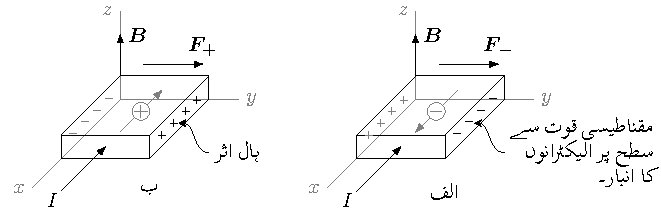
\includegraphics{figInductanceHallEffect}
\caption{ہال اثر سے متحرک چارج کا قطب دریافت کیا جا سکتا ہے۔}
\label{شکل_امالہ_ہال_قطب_کا_حصول}
\end{figure}

مثبت آئن اور منفی الیکٹران کے مابین کولمب قوتیں انتہائی طاقتور ہوتی ہیں لہٰذا مقناطیسی میدان سے پیدا فاصلوں میں تبدیلی قابل ناپ نہیں ہوتی۔مثبت اور منفی چارجوں کے مابین فاصلے کی بنا پر انہیں دو چادر کپیسٹر تصور کیا جا سکتا ہے۔ہم جانتے ہیں کہ ایسے کپیسٹر کے چادروں کے مابین برقی دباو پایا جاتا ہے۔یوں الیکٹران کے حرکت اور مقناطیسی میدان دونوں کی سمتوں کے عمودی دو الٹ اطراف کے مابین تار پر معمولی برقی دباو پایا جاتا ہے جسے \اصطلاح{ہال اثر}\فرہنگ{ہال!اثر}\حاشیہب{Hall effect}\فرہنگ{Hall!effect} کے نام\حاشیہد{ایڈون حال نے اس اثر کو  1879 میں دریافت کیا۔} سے جانا جاتا ہے۔

ہال اثر کو شکل \حوالہ{شکل_امالہ_ہال_قطب_کا_حصول} کی مدد سے باآسانی سمجھا جا سکتا ہے۔شکل-الف میں موصل یا \عددیء{n} قسم کے نیم موصل برقی رو گزارتا تار دکھایا گیا ہے۔تار میں برقی رو \عددیء{I} کی سمت \عددیء{-\ax} ہے  لہٰذا تار میں آزاد منفی چارج اس کے الٹ یعنی \عددیء{\ax} سمت  میں حرکت کر رہے ہیں۔تار میں آزاد الیکٹران کو ہلکی سیاہی میں تیر کے نشان پر دائرے میں بند \عددیء{-} علامت سے ظاہر کیا گیا ہے جہاں تیر اس کے حرکت کی سمت ظاہر کرتا ہے۔یہ تار \عددیء{\az} سمت کے مقناطیسی میدان میں پڑی ہے۔تار میں آزاد چارج منفی قطب کے ہیں لہٰذا ان پر مساوات \حوالہ{مساوات_امالہ_مقناطیسی_قوت} کے تحت \عددیء{\ay} سمت میں قوت \عددیء{\kvec{F_-}} عمل کرے گا۔قوت کی علامت پر زیر نوشت میں منفی کی علامت یہ ظاہر کرتی ہے کہ یہ قوت متحرک منفی چارج پر اثر انداز ہوتا ہے۔یوں تار کے دائیں طرف پر منفی الیکٹرانوں کا انبار جمع ہوتا ہے جبکہ تار کے بائیں طرف پر الیکٹران کی تعداد کم ہو جاتی ہے جس سے اس جانب ساکن مثبت آئن \اصطلاح{بے پردہ}\فرہنگ{بے پردہ}\حاشیہب{uncovered}\فرہنگ{charges!uncovered} ہو جاتے ہیں۔شکل \حوالہ{شکل_امالہ_ہال_قطب_کا_حصول}-الف میں تار کے دائیں طرف \عددیء{-} اور بائیں طرف  \عددیء{+} کے علامات انہیں کو ظاہر کرتے ہیں۔آپ جانتے ہیں کہ مثبت اور  منفی چارج  کے مابین برقی میدان کی شدت \عددیء{\kvec{E}} اور یوں برقی دباو پایا جاتا ہے لہٰذا تار کے دائیں اور بائیں اطراف کے مابین \اصطلاح{ہال برقی دباو}\فرہنگ{ہال!برقی دباو}\حاشیہب{Hall voltage}\فرہنگ{Hall!voltage} پایا جائے گا۔تار کا بایاں طرف ہال برقی دباو کا مثبت سرا ہو گا۔

آئیں ایسی صورت دیکھیں جہاں متحرک مثبت چارج کی بدولت برقی رو پائی جائے۔شکل \حوالہ{شکل_امالہ_ہال_قطب_کا_حصول}-ب میں بقایا صورت حال بالکل شکل-الف کی طرح ہے البتہ یہاں تار \عددیء{p} قسم کے نیم موصل کا بنا ہوا ہے جس میں برقی رو مثبت \اصطلاح{آزاد خول}\فرہنگ{خول!آزاد}\حاشیہب{free holes}\فرہنگ{holes!free} کے حرکت سے پیدا ہوتی ہے۔یوں اگر برقی رو \عددیء{-\ax} سمت میں ہو تب آزاد خول بھی اسی سمت میں حرکت کریں گے۔جیسے شکل میں دکھایا گیا ہے یہاں بھی مقناطیسی قوت آزاد چارج کو دائیں جانب دھکیل رہے ہیں۔آپ دیکھ سکتے ہیں کہ اس بار ہال برقی دباو کا مثبت سرا تار کا دائیں طرف پایا جاتا ہے جو شکل-الف کے عین الٹ ہے۔اس حقیقت کو استعمال کرتے ہوئے یہ معلوم کیا جا سکتا ہے کہ آیا  نیم موصل \عددیء{n} یا \عددیء{p} قسم کا ہے۔

ہال اثر استعمال کرتے ہوئے مختلف پیمائشی آلات بنائے جاتے ہیں مثلاً \اصطلاح{یک سمتی رو پیما}\فرہنگ{ہال!یک سمتی رو پیما}\فرہنگ{Hall!effect current meter}، \اصطلاح{مقناطیسی بہاو پیما}\فرہنگ{ہال_مقناطیسی بہاو پیما}\حاشیہب{magnetic flux meter}\فرہنگ{Hall!magnetic flux meter} وغیرہ۔

سمتی رفتار \عددیء{\kvec{v}} سے حرکت کرتا ہوا حجمی کثافت چارج \عددیء{\rho_h}  کثافت برقی رو \عددیء{\kvec{J}}
\begin{align}
\kvec{J}=\rho_h \kvec{v}
\end{align}
کو جنم دیتا ہے۔اس مساوات کو صفحہ \حوالہصفحہ{مساوات_کپیسٹر_کثافت_رو_مساوی_کثافت_چارج_ضرب_رفتار} پر حاصل کیا گیا۔چھوٹے حجم \عددیء{\dif h} میں تھوڑے سے چارج کو
\begin{align}
\dif Q=\rho_h \dif h
\end{align}
لکھا جا سکتا ہے لہٰذا مساوات \حوالہ{مساوات_امالہ_مقناطیسی_تفرقی_قوت} کو
\begin{align*}
\dif \kvec{F}=\rho_h \dif h \kvec{v} \times \kvec{B}
\end{align*}
یا
\begin{align}\label{مساوات_امالہ_لورنز_تفرقی_الف}
\dif \kvec{F}=\kvec{J} \times \kvec{B} \dif h
\end{align}
لکھا جا سکتا ہے۔ہم پہلے دیکھ چکے ہیں کہ \عددیء{\kvec{J} \dif h} کو تفرقی برقی رو گزارتے تار کا حصہ تصور کیا جا سکتا ہے جسے یوں
\begin{align*}
\kvec{J} \dif h=\kvec{K} \dif S=I \dif \kvec{L}
\end{align*}
بھی لکھا جا سکتا ہے۔اس طرح مساوات \حوالہ{مساوات_امالہ_لورنز_تفرقی_الف} کو
\begin{align}\label{مساوات_امالہ_لورنز_تفرقی_ب}
\dif \kvec{F}=\kvec{K} \times \kvec{B} \dif S
\end{align}
یا 
\begin{align}\label{مساوات_امالہ_لورنز_تفرقی_پ}
\dif \kvec{F}=I \dif \kvec{L} \times \kvec{B}
\end{align}
بھی لکھا جا سکتا ہے۔

مساوات \حوالہ{مساوات_امالہ_لورنز_تفرقی_الف}، مساوات \حوالہ{مساوات_امالہ_لورنز_تفرقی_ب} اور مساوات \حوالہ{مساوات_امالہ_لورنز_تفرقی_پ} کے تکمل سے انہیں یوں
\begin{align}
\kvec{F}&=\int_h \kvec{J} \times \kvec{B} \dif h\\
\kvec{F}&=\int_S \kvec{K} \times \kvec{B} \dif S\\
\kvec{F}&=\oint I \dif \kvec{L} \times \kvec{B} \label{مساوات_امالہ_لورنز_تتکمل_پ}
\end{align}
لکھا جا سکتا ہے۔

مساوات \حوالہ{مساوات_امالہ_لورنز_تتکمل_پ} میں اگر \عددیء{L} لمبائی کی سیدھی تار لی جائے تو تکمل سے
\begin{align}\label{مساوات_امالہ_سیدھی_تار_قوت_الف}
\kvec{F}=I \kvec{L} \times \kvec{B}
\end{align}
حاصل ہوتا ہے جس میں قوت کی قیمت
\begin{align}\label{مساوات_امالہ_سیدھی_تار_قوت_ب}
F=I L B \sin \theta
\end{align}
ہے جہاں تار اور مقناطیسی میدان کے درمیان زاویہ \عددیء{\theta} ہے۔مساوات \حوالہ{مساوات_امالہ_سیدھی_تار_قوت_الف} اور مساوات \حوالہ{مساوات_امالہ_سیدھی_تار_قوت_ب} پورے دور کے کچھ حصے پر قوت دیتے ہیں۔کسی بھی مسئلے میں پورے دور کا تکمل ضروری ہو گا۔
